\chapter{Protocolo de investigación}

\section{Introducción y antecendentes}
Los Algoritmos Evolutivos (Evolutionary Algorithms --- \EAS{}) son considerados como uno de los enfoques con mayor eficacia para resolver distintas categorías de 
problemas de optimización.
%
Se han desarrollado diversas variantes que han sido aplicadas en múltiples campos, como en transporte, economía o ingeniería.
%
Particularmente, se han aplicado tanto en problemas del dominio continuo (\cite{glover2005handbook}) como del dominio discreto (\cite{Joel:Dynamic_FAP}).
%
En general, los \EAS{} han sido especialmente exitosos en la resolución de problemas complejos en donde los enfoques exactos no son actualmente aplicables, como por ejemplo, en problemas NP-completos con espacios de búsqueda grandes (\cite{chakraborty2008advances}).
% 
\subsection{Optimizadores estocásticos poblacionales}

De acuerdo a \cite{voss2012meta}, una meta-heurística es un proceso maestro iterativo que guía y modifica las operaciones para ordenar heurísticas con el fin de producir de forma eficiente soluciones de calidad. 
%
Esto podría manipular una solución completa (o incompleta) o un conjunto de soluciones por iteración.
%
Las heurísticas subordinadas podrían ser prodecimientos de alto o bajo nivel, una búsqueda local simple, o un método constructivo.
%
Además, algunas de las clasificaciones bastante utilizadas en la literatura son (\cite{beheshti2013review}):
\begin{itemize}
    \item Inspirado en la naturaleza y no-inspirado en la naturaleza.
    \item En base a la población y en base a un simple punto.
\end{itemize}

Un panorama más amplio es mostrado en la figura \ref{fig:clasificacion}, este trabajo se enfoca principalmente a las meta-heurísticas poblacionales.
%
Las meta-heurísticas poblacionales son aquellas que utiliza múltiples soluciones en cada momento, otra caracterización es que este tipo de algoritmos realizan una búsqueda con múltiples puntos iniciales.
%
Algunas de las metaheurísticas poblacionales mas populares se listan a continuacón
\begin{itemize}
    \item Algoritmos genéticos (Genetic algorithm).
    \item Programación genética (Genetic programming).
    \item Programación evolutiva (Evolutionary programming).
    \item Evolución diferencial (Differential evolution).
    \item Búsqueda de dispersión (Scatter search).
    \item Estrategia evolutiva (Evolution strategy).
    \item Algoritmos de estimación de distribución (Estimation of distribution algorithm).
    \item Recocido simulado (Simulated annealing).
    \item Optimización por enjambre de partículas (Particle Swarm optimization).
    \item Algoritmos de optimización por colonias de hormigas (Ant colony optimization algorithms).
\end{itemize}

\begin{figure}[H]
\centering
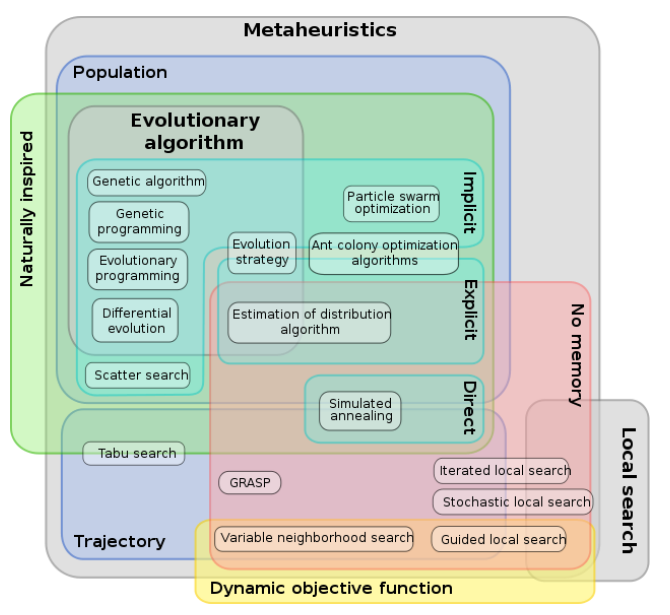
\includegraphics[width=0.8\textwidth]{clasificacion.png}
\caption{Clasificación del campo de meta-heurísticas. Figura tomada de \cite{beheshti2013review}.}
\label{fig:clasificacion}
\end{figure}



\subsection{Definición del problema}

Actualmente, los algoritmos evolutivos son una de las meta-heurísticas más conocidas (\cite{glover2005handbook}), pero a pesar de su éxito la mayoría son diagnosticados con problemas de convergencia acelerada, en consecuencia el proceso de búsqueda puede estar estancado al inicio de su tiempo total de ejecución y desperdiciar recursos valiosos el resto de su ejecución.
%
Este problema es más notorio al considerar ejecuciones a largo plazo y con problemas complejos.
%
Es por esto que adaptar estas meta-heurísticas a nuevos problemas implica la toma de varias decisiones de diseño complejas.
%
\subsection{Principios de diseño de un algoritmo estocástico poblacional}

Particularmente, a la hora de diseñar de forma apropiada un algoritmo evolutivo, se ha visto que es muy importante conseguir inducir un balanceo adecuado entre la exploración e intensificación del espacio de búsqueda (\cite{herrera1996adaptation}).
%
Nótese en este punto que, de manera informal, la exploración del espacio de búsqueda consiste en evaluar regiones del espacio de búsqueda que no han sido muestreadas con el fin de detectar regiones promisorias, y la explotación consiste en muestrear en zonas ya evaluadas previamente para realizar una búsqueda más profunda con el fin de encontrar soluciones más refinadas y de mayor calidad.
%
Cuando en los algoritmos evolutivos todas o casi todas las soluciones están en regiones distantes --- alta diversidad --- se produce habitualmente una búsqueda exploratoria, 
es decir, muchas de las nuevas soluciones evaluadas serán distantes a las ya evaluadas anteriormente.
%
Sin embargo, cuando casi todas las soluciones están en una o en unas pocas regiones, se produce una búsqueda intensificadora.
%
Uno de los problemas en el diseño de los algoritmos evolutivos es que en muchos casos no se comprenden todas las implicaciones que los diferentes componentes tienen sobre el mantenimiento de la diversidad de la población y en consecuencia sobre el balanceo entre exploración e intensificación (\cite{Crepinsek:13}).
%
Por ello, analizar el comportamiento y rediseñar en base a lo que está ocurriendo en este aspecto, es parte del proceso de diseño de los algoritmos evolutivos.

Relacionado con lo anterior, aparece el concepto de convergencia prematura (\cite{Crepinsek:13}).
%
Se dice que un algoritmo converge de forma prematura cuando mucho antes de alcanzar el criterio de paro, todas las soluciones están en una zona muy pequeña del espacio de búsqueda.
%
En este sentido, a partir de ese momento es difícil seguir mejorando las soluciones de forma significativa ya que con alta probabilidad sólo se va a realizar un muestreo de soluciones en dicha región.
%
Por ello, es importante detectar si esto ocurre y en tal caso rediseñar algunos aspectos del algoritmo para preservar una mayor diversidad.
%
Sin embargo, si la población es muy diversa durante todo el proceso de búsqueda, se podría no alcanzar un grado adecuado de intensificación y por lo tanto se tendría una convergencia lenta que posiblemente también resultaría en soluciones de baja calidad.

\subsection{Importancia de la diversidad, criterio de parada y tiempo transcurrido en optimización combinatoria}

En los últimos años, algunos de los trabajos más exitosos en el área de optimización combinatoria mono-objetivo son contemplados en ejecuciones a largo plazo y consideran mecanismos para gestionar diversidad de forma explícita en el espacio de las variables considerando el tiempo transcurrido y el criterio de parada.
%
Este tipo de métodos han encontrado los mejores resultados en varios problemas de combinatoria conocidos, como es el problema de asignación de frecuencias \citetitle{Joel:Dynamic_FAP} (\cite{Joel:Dynamic_FAP}), el problema del Sudoku \citetitle{Joel:Dynamic_Sudoku} (\cite{Joel:Dynamic_Sudoku}), el problema del agente viajero \citetitle{Joel:ANovelDiversityBasedEAForTheTSP} (\cite{Joel:ANovelDiversityBasedEAForTheTSP}), el problema de particionado de grafos \citetitle{romero2018memetic} (\cite{romero2018memetic}), el problema de embalaje bidimensional \citetitle{segredo2014memetic} (\cite{segredo2014memetic})  entre otros.

%para tratar el problema de convergencia prematura se han basado en considerar el criterio de parada y tiempo
%transcurrido para balancear entre exploración e intensificación~\cite{segura2016novel}.
%
%Esto se fundamenta en la premisa de que el grado entre exploración e intensificación debería variar a lo largo de la ejecución, por lo tanto tiene sentido que las decisiones tomadas por las componentes varíen en función del instante de ejecución.
%
%


